% Primes p = 1 mod 3 below 1200; dark if p = x^2+27y^2 (generated by a script).
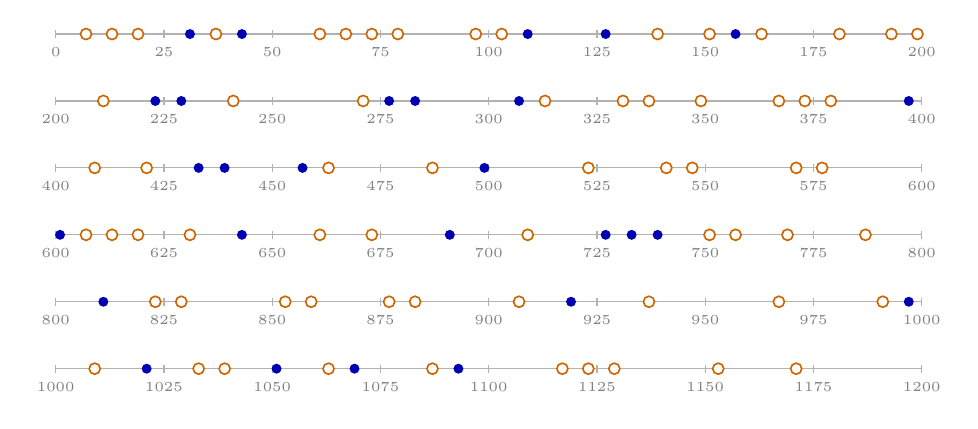
\begin{tikzpicture}[x=0.055cm,y=0.85cm]
\draw[black!30] (0,0)--(200,0);
\draw[black!30] (0,0-0.06)--(0,0+0.06);
\node[font=\tiny,black!50,below] at (0,0-0.06) {0};
\draw[black!30] (25,0-0.06)--(25,0+0.06);
\node[font=\tiny,black!50,below] at (25,0-0.06) {25};
\draw[black!30] (50,0-0.06)--(50,0+0.06);
\node[font=\tiny,black!50,below] at (50,0-0.06) {50};
\draw[black!30] (75,0-0.06)--(75,0+0.06);
\node[font=\tiny,black!50,below] at (75,0-0.06) {75};
\draw[black!30] (100,0-0.06)--(100,0+0.06);
\node[font=\tiny,black!50,below] at (100,0-0.06) {100};
\draw[black!30] (125,0-0.06)--(125,0+0.06);
\node[font=\tiny,black!50,below] at (125,0-0.06) {125};
\draw[black!30] (150,0-0.06)--(150,0+0.06);
\node[font=\tiny,black!50,below] at (150,0-0.06) {150};
\draw[black!30] (175,0-0.06)--(175,0+0.06);
\node[font=\tiny,black!50,below] at (175,0-0.06) {175};
\draw[black!30] (200,0-0.06)--(200,0+0.06);
\node[font=\tiny,black!50,below] at (200,0-0.06) {200};
\draw[black!30] (0,-1)--(200,-1);
\draw[black!30] (0,-1-0.06)--(0,-1+0.06);
\node[font=\tiny,black!50,below] at (0,-1-0.06) {200};
\draw[black!30] (25,-1-0.06)--(25,-1+0.06);
\node[font=\tiny,black!50,below] at (25,-1-0.06) {225};
\draw[black!30] (50,-1-0.06)--(50,-1+0.06);
\node[font=\tiny,black!50,below] at (50,-1-0.06) {250};
\draw[black!30] (75,-1-0.06)--(75,-1+0.06);
\node[font=\tiny,black!50,below] at (75,-1-0.06) {275};
\draw[black!30] (100,-1-0.06)--(100,-1+0.06);
\node[font=\tiny,black!50,below] at (100,-1-0.06) {300};
\draw[black!30] (125,-1-0.06)--(125,-1+0.06);
\node[font=\tiny,black!50,below] at (125,-1-0.06) {325};
\draw[black!30] (150,-1-0.06)--(150,-1+0.06);
\node[font=\tiny,black!50,below] at (150,-1-0.06) {350};
\draw[black!30] (175,-1-0.06)--(175,-1+0.06);
\node[font=\tiny,black!50,below] at (175,-1-0.06) {375};
\draw[black!30] (200,-1-0.06)--(200,-1+0.06);
\node[font=\tiny,black!50,below] at (200,-1-0.06) {400};
\draw[black!30] (0,-2)--(200,-2);
\draw[black!30] (0,-2-0.06)--(0,-2+0.06);
\node[font=\tiny,black!50,below] at (0,-2-0.06) {400};
\draw[black!30] (25,-2-0.06)--(25,-2+0.06);
\node[font=\tiny,black!50,below] at (25,-2-0.06) {425};
\draw[black!30] (50,-2-0.06)--(50,-2+0.06);
\node[font=\tiny,black!50,below] at (50,-2-0.06) {450};
\draw[black!30] (75,-2-0.06)--(75,-2+0.06);
\node[font=\tiny,black!50,below] at (75,-2-0.06) {475};
\draw[black!30] (100,-2-0.06)--(100,-2+0.06);
\node[font=\tiny,black!50,below] at (100,-2-0.06) {500};
\draw[black!30] (125,-2-0.06)--(125,-2+0.06);
\node[font=\tiny,black!50,below] at (125,-2-0.06) {525};
\draw[black!30] (150,-2-0.06)--(150,-2+0.06);
\node[font=\tiny,black!50,below] at (150,-2-0.06) {550};
\draw[black!30] (175,-2-0.06)--(175,-2+0.06);
\node[font=\tiny,black!50,below] at (175,-2-0.06) {575};
\draw[black!30] (200,-2-0.06)--(200,-2+0.06);
\node[font=\tiny,black!50,below] at (200,-2-0.06) {600};
\draw[black!30] (0,-3)--(200,-3);
\draw[black!30] (0,-3-0.06)--(0,-3+0.06);
\node[font=\tiny,black!50,below] at (0,-3-0.06) {600};
\draw[black!30] (25,-3-0.06)--(25,-3+0.06);
\node[font=\tiny,black!50,below] at (25,-3-0.06) {625};
\draw[black!30] (50,-3-0.06)--(50,-3+0.06);
\node[font=\tiny,black!50,below] at (50,-3-0.06) {650};
\draw[black!30] (75,-3-0.06)--(75,-3+0.06);
\node[font=\tiny,black!50,below] at (75,-3-0.06) {675};
\draw[black!30] (100,-3-0.06)--(100,-3+0.06);
\node[font=\tiny,black!50,below] at (100,-3-0.06) {700};
\draw[black!30] (125,-3-0.06)--(125,-3+0.06);
\node[font=\tiny,black!50,below] at (125,-3-0.06) {725};
\draw[black!30] (150,-3-0.06)--(150,-3+0.06);
\node[font=\tiny,black!50,below] at (150,-3-0.06) {750};
\draw[black!30] (175,-3-0.06)--(175,-3+0.06);
\node[font=\tiny,black!50,below] at (175,-3-0.06) {775};
\draw[black!30] (200,-3-0.06)--(200,-3+0.06);
\node[font=\tiny,black!50,below] at (200,-3-0.06) {800};
\draw[black!30] (0,-4)--(200,-4);
\draw[black!30] (0,-4-0.06)--(0,-4+0.06);
\node[font=\tiny,black!50,below] at (0,-4-0.06) {800};
\draw[black!30] (25,-4-0.06)--(25,-4+0.06);
\node[font=\tiny,black!50,below] at (25,-4-0.06) {825};
\draw[black!30] (50,-4-0.06)--(50,-4+0.06);
\node[font=\tiny,black!50,below] at (50,-4-0.06) {850};
\draw[black!30] (75,-4-0.06)--(75,-4+0.06);
\node[font=\tiny,black!50,below] at (75,-4-0.06) {875};
\draw[black!30] (100,-4-0.06)--(100,-4+0.06);
\node[font=\tiny,black!50,below] at (100,-4-0.06) {900};
\draw[black!30] (125,-4-0.06)--(125,-4+0.06);
\node[font=\tiny,black!50,below] at (125,-4-0.06) {925};
\draw[black!30] (150,-4-0.06)--(150,-4+0.06);
\node[font=\tiny,black!50,below] at (150,-4-0.06) {950};
\draw[black!30] (175,-4-0.06)--(175,-4+0.06);
\node[font=\tiny,black!50,below] at (175,-4-0.06) {975};
\draw[black!30] (200,-4-0.06)--(200,-4+0.06);
\node[font=\tiny,black!50,below] at (200,-4-0.06) {1000};
\draw[black!30] (0,-5)--(200,-5);
\draw[black!30] (0,-5-0.06)--(0,-5+0.06);
\node[font=\tiny,black!50,below] at (0,-5-0.06) {1000};
\draw[black!30] (25,-5-0.06)--(25,-5+0.06);
\node[font=\tiny,black!50,below] at (25,-5-0.06) {1025};
\draw[black!30] (50,-5-0.06)--(50,-5+0.06);
\node[font=\tiny,black!50,below] at (50,-5-0.06) {1050};
\draw[black!30] (75,-5-0.06)--(75,-5+0.06);
\node[font=\tiny,black!50,below] at (75,-5-0.06) {1075};
\draw[black!30] (100,-5-0.06)--(100,-5+0.06);
\node[font=\tiny,black!50,below] at (100,-5-0.06) {1100};
\draw[black!30] (125,-5-0.06)--(125,-5+0.06);
\node[font=\tiny,black!50,below] at (125,-5-0.06) {1125};
\draw[black!30] (150,-5-0.06)--(150,-5+0.06);
\node[font=\tiny,black!50,below] at (150,-5-0.06) {1150};
\draw[black!30] (175,-5-0.06)--(175,-5+0.06);
\node[font=\tiny,black!50,below] at (175,-5-0.06) {1175};
\draw[black!30] (200,-5-0.06)--(200,-5+0.06);
\node[font=\tiny,black!50,below] at (200,-5-0.06) {1200};
\draw[orange!80!black,line width=0.6pt,fill=white] (7,0) circle (2pt);
\draw[orange!80!black,line width=0.6pt,fill=white] (13,0) circle (2pt);
\draw[orange!80!black,line width=0.6pt,fill=white] (19,0) circle (2pt);
\fill[blue!70!black] (31,0) circle (1.8pt);
\draw[orange!80!black,line width=0.6pt,fill=white] (37,0) circle (2pt);
\fill[blue!70!black] (43,0) circle (1.8pt);
\draw[orange!80!black,line width=0.6pt,fill=white] (61,0) circle (2pt);
\draw[orange!80!black,line width=0.6pt,fill=white] (67,0) circle (2pt);
\draw[orange!80!black,line width=0.6pt,fill=white] (73,0) circle (2pt);
\draw[orange!80!black,line width=0.6pt,fill=white] (79,0) circle (2pt);
\draw[orange!80!black,line width=0.6pt,fill=white] (97,0) circle (2pt);
\draw[orange!80!black,line width=0.6pt,fill=white] (103,0) circle (2pt);
\fill[blue!70!black] (109,0) circle (1.8pt);
\fill[blue!70!black] (127,0) circle (1.8pt);
\draw[orange!80!black,line width=0.6pt,fill=white] (139,0) circle (2pt);
\draw[orange!80!black,line width=0.6pt,fill=white] (151,0) circle (2pt);
\fill[blue!70!black] (157,0) circle (1.8pt);
\draw[orange!80!black,line width=0.6pt,fill=white] (163,0) circle (2pt);
\draw[orange!80!black,line width=0.6pt,fill=white] (181,0) circle (2pt);
\draw[orange!80!black,line width=0.6pt,fill=white] (193,0) circle (2pt);
\draw[orange!80!black,line width=0.6pt,fill=white] (199,0) circle (2pt);
\draw[orange!80!black,line width=0.6pt,fill=white] (11,-1) circle (2pt);
\fill[blue!70!black] (23,-1) circle (1.8pt);
\fill[blue!70!black] (29,-1) circle (1.8pt);
\draw[orange!80!black,line width=0.6pt,fill=white] (41,-1) circle (2pt);
\draw[orange!80!black,line width=0.6pt,fill=white] (71,-1) circle (2pt);
\fill[blue!70!black] (77,-1) circle (1.8pt);
\fill[blue!70!black] (83,-1) circle (1.8pt);
\fill[blue!70!black] (107,-1) circle (1.8pt);
\draw[orange!80!black,line width=0.6pt,fill=white] (113,-1) circle (2pt);
\draw[orange!80!black,line width=0.6pt,fill=white] (131,-1) circle (2pt);
\draw[orange!80!black,line width=0.6pt,fill=white] (137,-1) circle (2pt);
\draw[orange!80!black,line width=0.6pt,fill=white] (149,-1) circle (2pt);
\draw[orange!80!black,line width=0.6pt,fill=white] (167,-1) circle (2pt);
\draw[orange!80!black,line width=0.6pt,fill=white] (173,-1) circle (2pt);
\draw[orange!80!black,line width=0.6pt,fill=white] (179,-1) circle (2pt);
\fill[blue!70!black] (197,-1) circle (1.8pt);
\draw[orange!80!black,line width=0.6pt,fill=white] (9,-2) circle (2pt);
\draw[orange!80!black,line width=0.6pt,fill=white] (21,-2) circle (2pt);
\fill[blue!70!black] (33,-2) circle (1.8pt);
\fill[blue!70!black] (39,-2) circle (1.8pt);
\fill[blue!70!black] (57,-2) circle (1.8pt);
\draw[orange!80!black,line width=0.6pt,fill=white] (63,-2) circle (2pt);
\draw[orange!80!black,line width=0.6pt,fill=white] (87,-2) circle (2pt);
\fill[blue!70!black] (99,-2) circle (1.8pt);
\draw[orange!80!black,line width=0.6pt,fill=white] (123,-2) circle (2pt);
\draw[orange!80!black,line width=0.6pt,fill=white] (141,-2) circle (2pt);
\draw[orange!80!black,line width=0.6pt,fill=white] (147,-2) circle (2pt);
\draw[orange!80!black,line width=0.6pt,fill=white] (171,-2) circle (2pt);
\draw[orange!80!black,line width=0.6pt,fill=white] (177,-2) circle (2pt);
\fill[blue!70!black] (1,-3) circle (1.8pt);
\draw[orange!80!black,line width=0.6pt,fill=white] (7,-3) circle (2pt);
\draw[orange!80!black,line width=0.6pt,fill=white] (13,-3) circle (2pt);
\draw[orange!80!black,line width=0.6pt,fill=white] (19,-3) circle (2pt);
\draw[orange!80!black,line width=0.6pt,fill=white] (31,-3) circle (2pt);
\fill[blue!70!black] (43,-3) circle (1.8pt);
\draw[orange!80!black,line width=0.6pt,fill=white] (61,-3) circle (2pt);
\draw[orange!80!black,line width=0.6pt,fill=white] (73,-3) circle (2pt);
\fill[blue!70!black] (91,-3) circle (1.8pt);
\draw[orange!80!black,line width=0.6pt,fill=white] (109,-3) circle (2pt);
\fill[blue!70!black] (127,-3) circle (1.8pt);
\fill[blue!70!black] (133,-3) circle (1.8pt);
\fill[blue!70!black] (139,-3) circle (1.8pt);
\draw[orange!80!black,line width=0.6pt,fill=white] (151,-3) circle (2pt);
\draw[orange!80!black,line width=0.6pt,fill=white] (157,-3) circle (2pt);
\draw[orange!80!black,line width=0.6pt,fill=white] (169,-3) circle (2pt);
\draw[orange!80!black,line width=0.6pt,fill=white] (187,-3) circle (2pt);
\fill[blue!70!black] (11,-4) circle (1.8pt);
\draw[orange!80!black,line width=0.6pt,fill=white] (23,-4) circle (2pt);
\draw[orange!80!black,line width=0.6pt,fill=white] (29,-4) circle (2pt);
\draw[orange!80!black,line width=0.6pt,fill=white] (53,-4) circle (2pt);
\draw[orange!80!black,line width=0.6pt,fill=white] (59,-4) circle (2pt);
\draw[orange!80!black,line width=0.6pt,fill=white] (77,-4) circle (2pt);
\draw[orange!80!black,line width=0.6pt,fill=white] (83,-4) circle (2pt);
\draw[orange!80!black,line width=0.6pt,fill=white] (107,-4) circle (2pt);
\fill[blue!70!black] (119,-4) circle (1.8pt);
\draw[orange!80!black,line width=0.6pt,fill=white] (137,-4) circle (2pt);
\draw[orange!80!black,line width=0.6pt,fill=white] (167,-4) circle (2pt);
\draw[orange!80!black,line width=0.6pt,fill=white] (191,-4) circle (2pt);
\fill[blue!70!black] (197,-4) circle (1.8pt);
\draw[orange!80!black,line width=0.6pt,fill=white] (9,-5) circle (2pt);
\fill[blue!70!black] (21,-5) circle (1.8pt);
\draw[orange!80!black,line width=0.6pt,fill=white] (33,-5) circle (2pt);
\draw[orange!80!black,line width=0.6pt,fill=white] (39,-5) circle (2pt);
\fill[blue!70!black] (51,-5) circle (1.8pt);
\draw[orange!80!black,line width=0.6pt,fill=white] (63,-5) circle (2pt);
\fill[blue!70!black] (69,-5) circle (1.8pt);
\draw[orange!80!black,line width=0.6pt,fill=white] (87,-5) circle (2pt);
\fill[blue!70!black] (93,-5) circle (1.8pt);
\draw[orange!80!black,line width=0.6pt,fill=white] (117,-5) circle (2pt);
\draw[orange!80!black,line width=0.6pt,fill=white] (123,-5) circle (2pt);
\draw[orange!80!black,line width=0.6pt,fill=white] (129,-5) circle (2pt);
\draw[orange!80!black,line width=0.6pt,fill=white] (153,-5) circle (2pt);
\draw[orange!80!black,line width=0.6pt,fill=white] (171,-5) circle (2pt);
\end{tikzpicture}
